\documentclass[12pt]{article}
\usepackage{amssymb,amsmath,latexsym}
\usepackage{graphicx}

% Page length commands go here in the preamble
\setlength{\oddsidemargin}{-0.25in}  % Left margin of 1 in + 0 in = 1 in
\setlength{\textwidth}{7in}  % Right margin of 8.5 in - 1 in - 6.5 in = 1 in
\setlength{\topmargin}{-.75in}  % Top margin of 2 in -0.75 in = 1 in
\setlength{\textheight}{9.2in}  % Lower margin of 11 in - 9 in - 1 in = 1 in

%\renewcommand{\baselinestretch}{1.5}  % 1.5 denotes double spacing. Changing it will change the spacing

\setlength{\parindent}{0in} 
\begin{document}
\title{CS 440 -- Intro to AI \\ Report 3: Heuristic Search}
\author{Skyler Malinowski (som12) \\ Andrew Dos Reis (ad1005)}
\date{December 6, 2017}
\maketitle

\newpage

\section{Part A}
% Show sample of interface
Our implementation makes use of a GUI and terminal to display relevant information. The GUI displays the map with color denoting what kind of cells they are and a path trace for the shortest path found. Whilest the terminal is used to display information regarding the cell that was clicked on. Of such information is the location of node \(n\), in programming notation, and the values corresponding to variables in \(f(n) = g(n) + h(n)\).

\section{Part B}
% (15 points)
\subsection{A*}
% Insert Example Solution with information
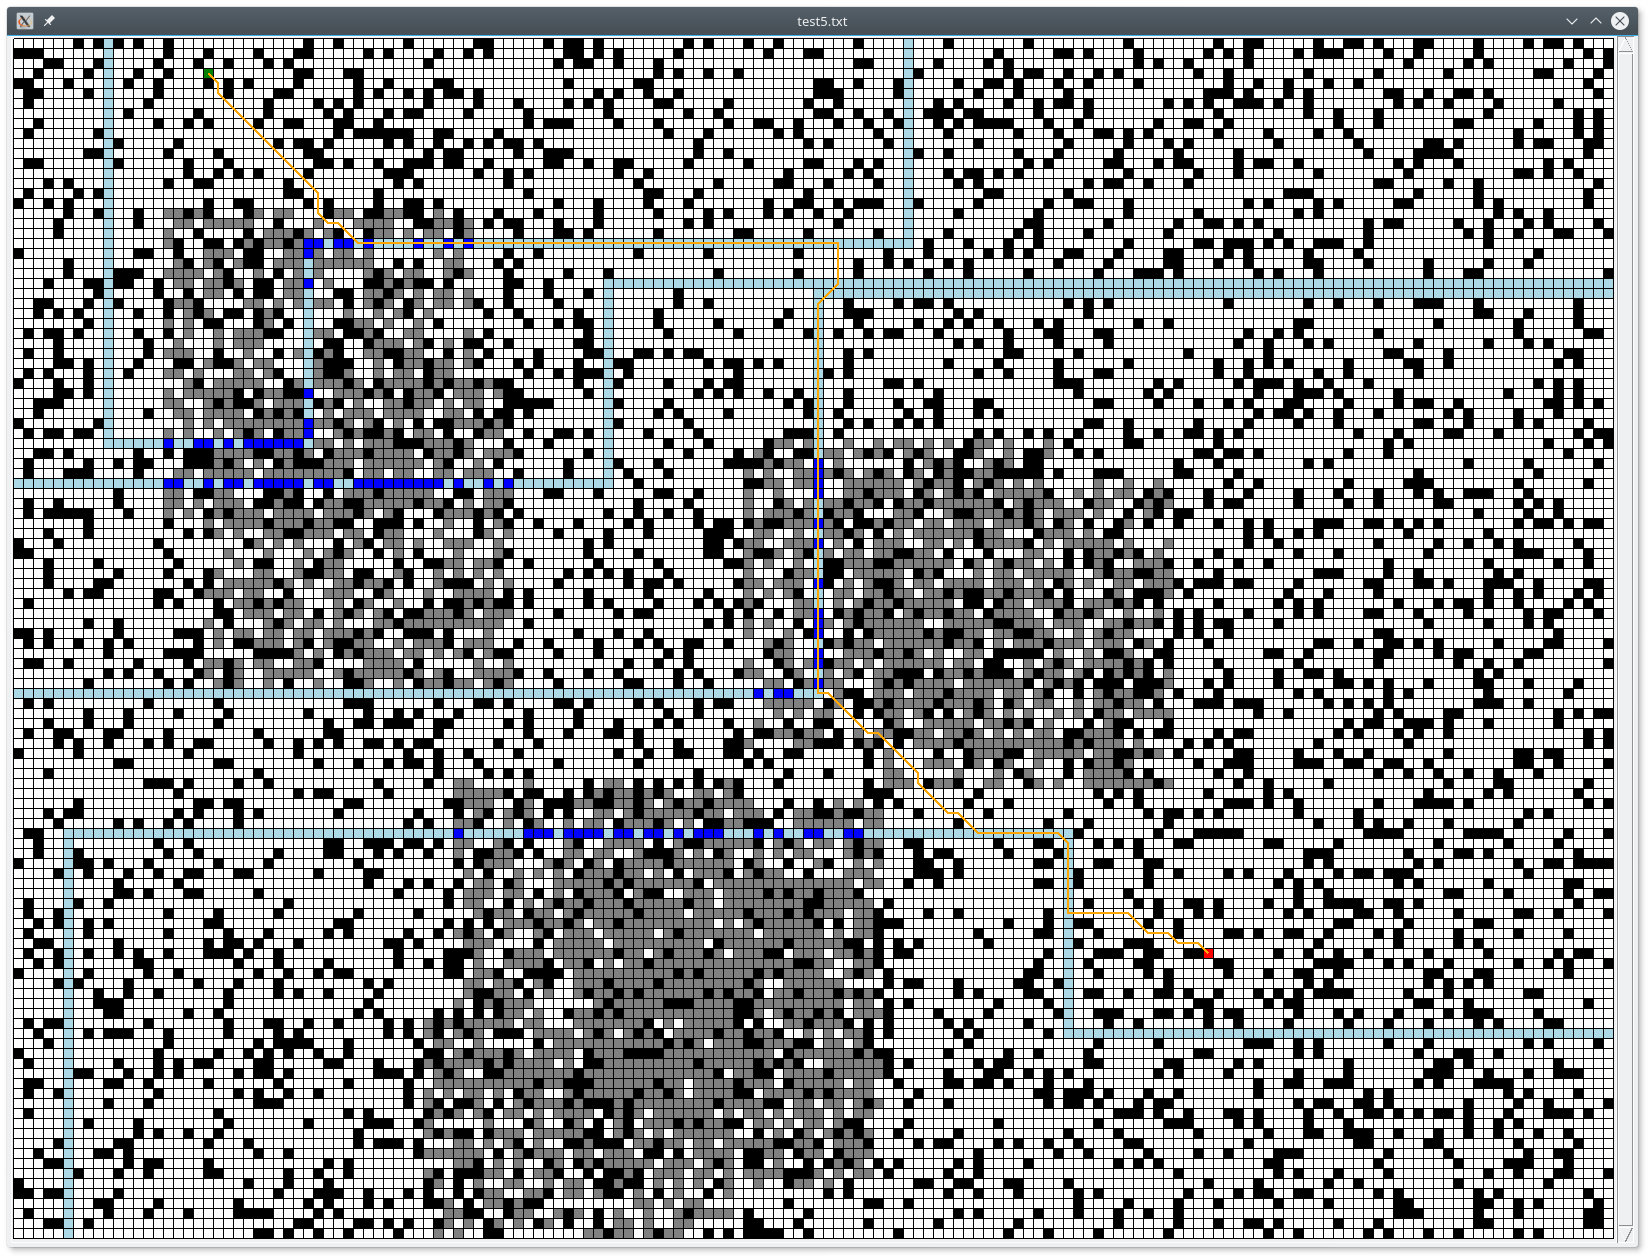
\includegraphics[scale=0.415]{aStar1.png}
\newline
Shortest Path Length: 99.27260094890539

\subsection{Weighted A*}
% Insert Example Solution with information
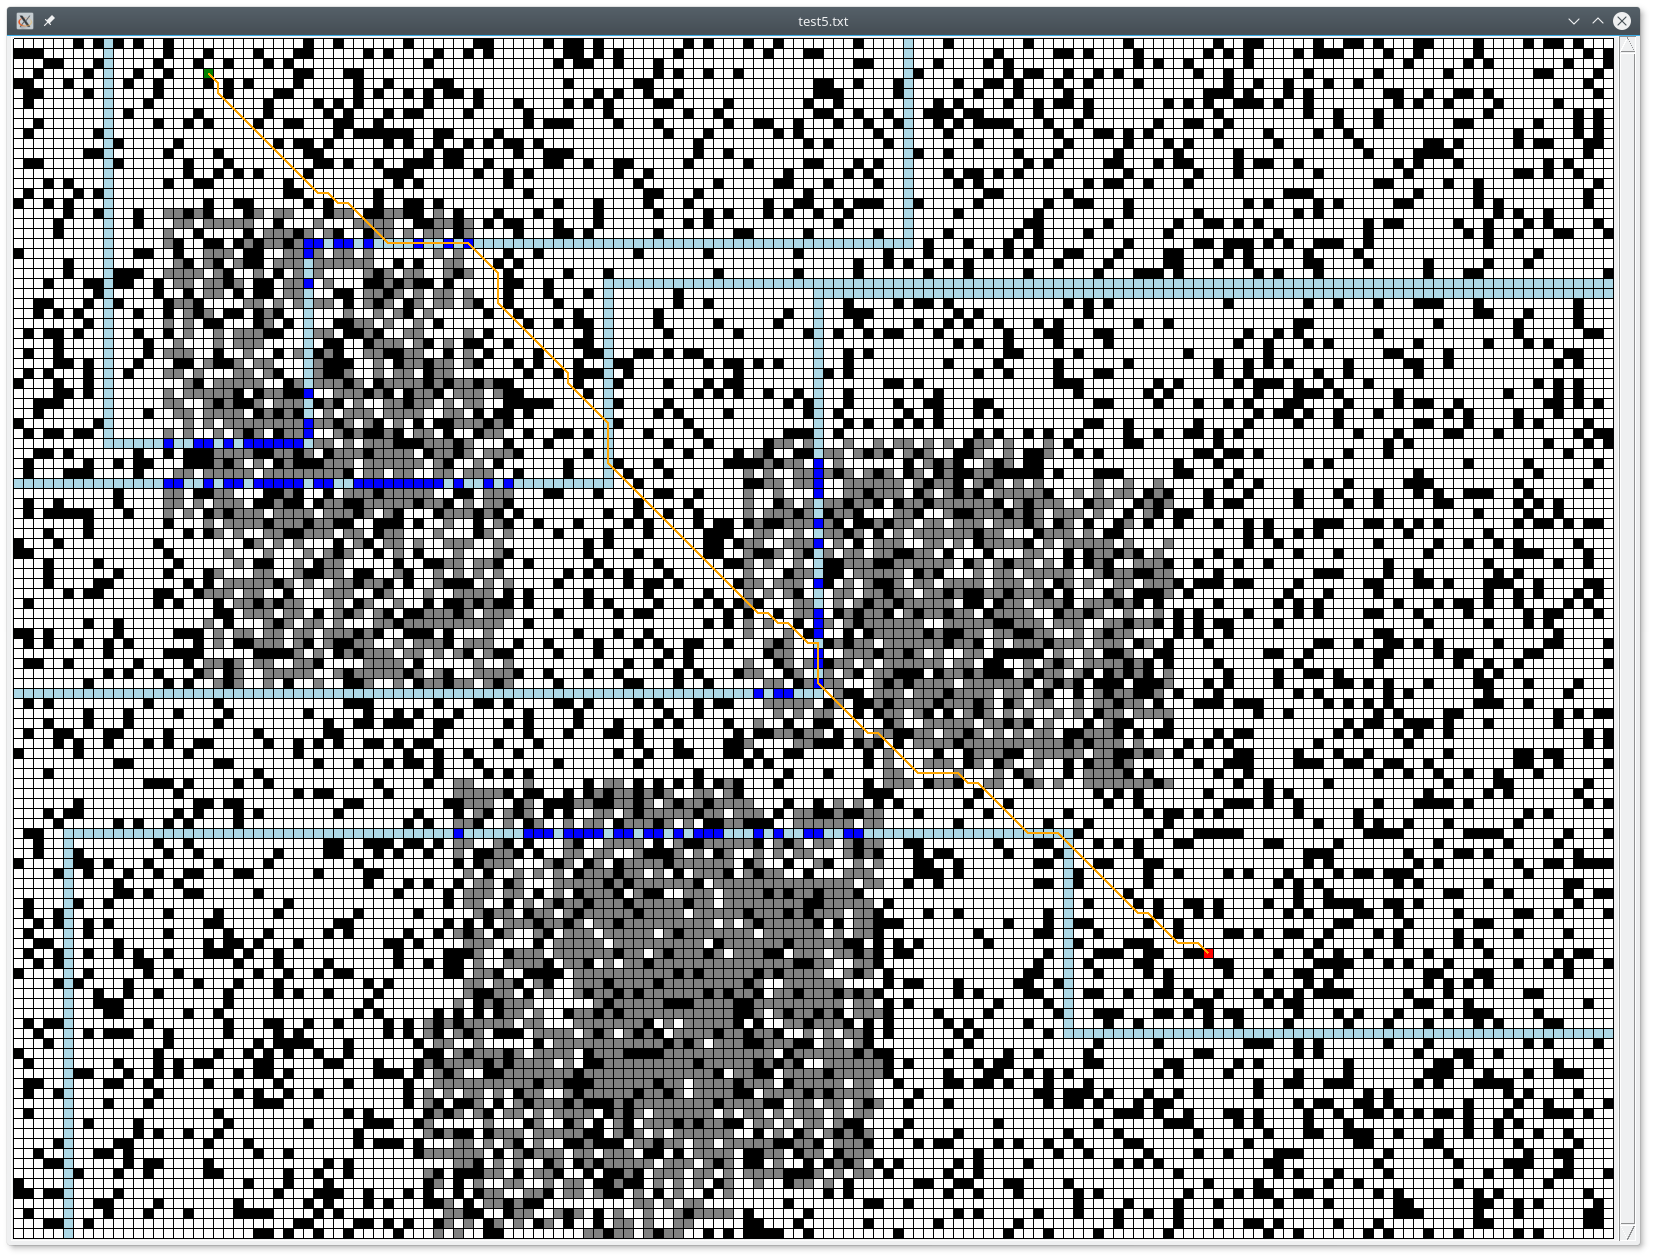
\includegraphics[scale=0.415]{W1_5_aStar1.png}
\newline
Shortest Path Length (\(w = 1.5\)): 138.07642481806775

\subsection{Uniform Cost Search}
% Insert Example Solution with information
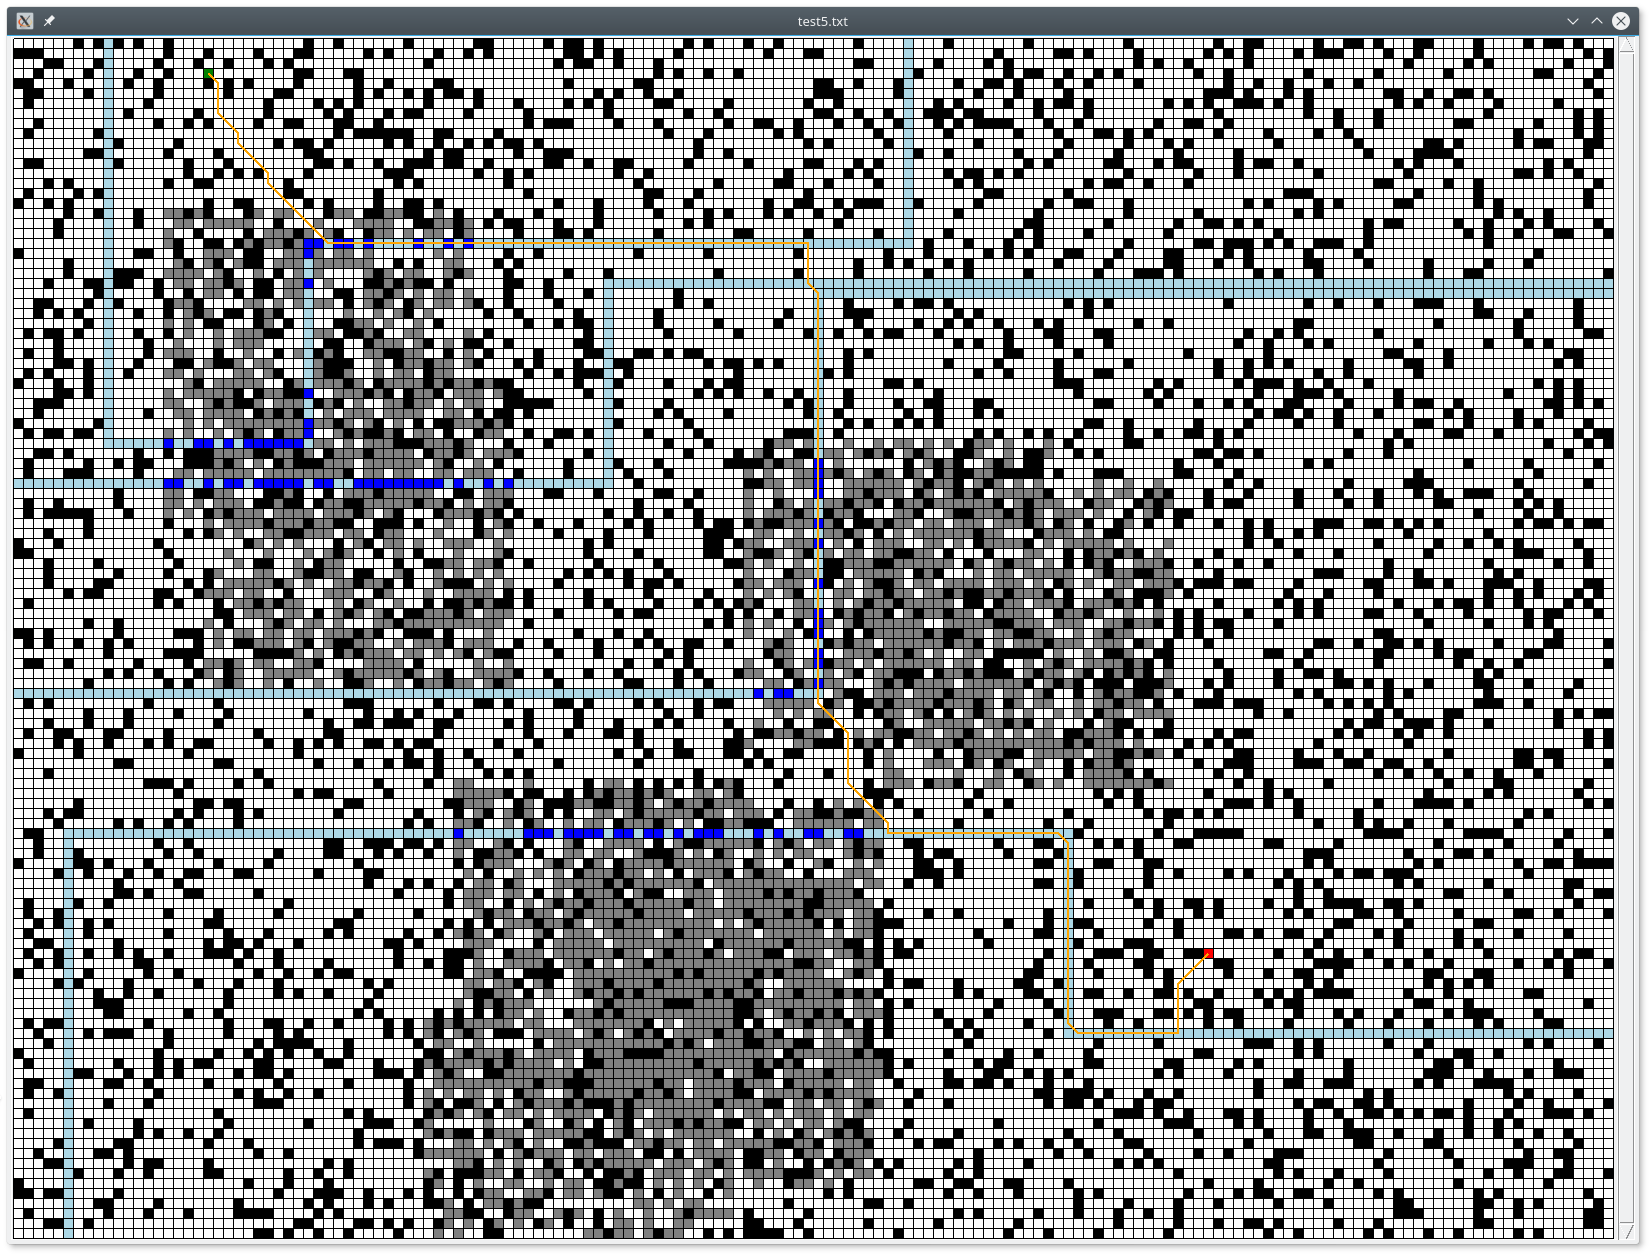
\includegraphics[scale=0.415]{Uniform1.png}
\newline
Shortest Path Length: 94.00178566873412

\section{Part C}
% Optimize your implementation of the above algorithms. Discuss your optimizations in your report. (10 points)
There are few points of optimality in context of pathfinding search algorithms.
\begin{itemize}
  \item A prioity queue on the open list with \(f(n)\) being the priority factor. This is to ensure that the algorithm is not uselessly expanding nodes that with higher probability will not lead to optimal solution. To do this we implemented the priority queue for the open list as a Binary Heap which naturally orders its contents in ascending order so that the first item popped off of the queue is the largest in value. This saves time and memory by not having to search through the open list to find the largest \(f(n)\) value.
  \item Making sure the heuristic does not overestimate. If it does, then the algorithm is no longer admissable as a heuristic, ergo the optimal path is no longer guaranteed. In an effort to ensure it never overestimates, the heuristic is modified by the best case movement cost for the world in question. For such a modification to actually result in an admissible heuristic the unmodified heuristic must agree on the degrees of freedom of movement of the agent for the world in question. 
\end{itemize}


\section{Part D}
% Propose different types of heuristics for the considered problem and discuss them in your report. In particular:
% • Propose the best admissible/consistent heuristic that you can come up with in this grid world.
% • Propose at least four other heuristics, which can be inadmissible but still useful for this problem and justify your choices.
% Remember that good heuristics can effectively guide the exploration process of a search algorithm towards finding a good solution fast and they are computationally inexpensive to compute. (10 points)
These are the Heuristics we implemented, where Modified indicates that it was multiplied by the lowest terrain travel cost coefficient and Raw means it is the standard implementation of that Heuristic without a coefficient
\subsection{Modified Euclidean Distance}
 \[ h = (0.25) * \sqrt{ (x_{current} - x_{goal})^2 + (y_{current} - y_{goal})^2}\]
\newline
 Admissible because it underestimates the distance to the goal by assuming that it will be traveling on river tiles the entire path and because it accounts for full freedom of movement for our agent
\subsection{Modified Chebyshev Distance}
  \[ h = (0.25) * \max( | x_{current} - x_{goal} |, | y_{current} - y_{goal} | )\]
\newline
Admissible because it underestimates the distance to the goal by assuming that it will be traveling on river tiles the entire path and because it accounts for full freedom of movement for our agent
\subsection{Modified Manhattan Distance}
\[ h = (0.25) * ( | x_{current} - x_{goal} | + | y_{current} - y_{goal} | )\]
\newline
Inadmissible because while it underestimates the distance to the goal by assuming that it will be traveling on river tiles the entire path it does not account for the full freedom of movement our agent has in our world
\subsection{Raw Chebyshev Distance}
 \[ h = \max( | x_{current} - x_{goal} |, | y_{current} - y_{goal} | )\]
\newline
Inadmissible because it does not underestimate the distance to the goal even though it does account for the full freedom of movement of our agent
\subsection{Raw Manhattan Distance}
\[ h =  ( | x_{current} - x_{goal} | + | y_{current} - y_{goal} | )\] 
Inadmissible because it does not underestimate the distance to the goal and it does not account for the full freedom of movement of our agent


\section{Part E}
% Perform an experimental evaluation on the 50 benchmarks using the three algorithms that you have implemented for the 5 different heuristics that you have considered. For Weighted A∗ you should try at least two w values, e.g., 1.25 and 2 (feel free to experiment). Compare the various solutions in terms of average run-time, average resulting path lengths as a function of the optimum length, average number of nodes expanded and memory requirements (average over all 50 benchmarks). In your report, provide your experimental results. (15 points)


\section{Part F}
% Explain your results and discuss in detail your observations regarding the relative performance of the different methods. What impact do you perceive that different heuristic functions have on the behavior of the algorithms and why? What is the relative performance of the different algorithms and why? (10 points)


\section{Part G}
% Implement the Sequential Heuristic A∗. Use an admissible heuristic for the anchor search. Use 4 other heuristics, admissible or inadmissible ones, for the remaining search processes. You should try at least two w1 and two w2 values, e.g., 1.25 and 2 (feel free to experiment). Make choices so as to optimize the performance of the algorithm, i.e., aim for solutions that compute as high-quality solutions and as fast as possible.
% Perform an experimental evaluation over the 50 benchmarks you have considered above. In particular, compare the A∗ approach with the admissible heuristic against the Sequential Heuristic version, which utilizes all the heuristics you have considered. Compare the various solutions in terms of average runtime, average resulting path lengths as a function of the optimum length, average number of nodes expanded and memory requirements (average over all 50 benchmarks). In your report, provide your experimental results. (15 points)


\section{Part H}
%  Describe in your report why your implementation is efficient. Explain your results and discuss in detail your observations regarding the relative performance of the methods. Discuss the relationship with your experiments for section e. What is the relative performance of the different algorithm in terms of computation time and solution quality and why? (10 points)


\section{Part I}
% Refer to Document for question (too long to put).


\end{document}